\documentclass[10pt,a4paper]{article}
\usepackage[margin=20mm]{geometry}
\usepackage[T1]{fontenc}
\usepackage{lmodern,graphicx,booktabs,array,xcolor,amsmath,siunitx,hyperref,float,caption}
\hypersetup{colorlinks=true,urlcolor=blue,linkcolor=blue}
\setlength{\parindent}{0pt}\setlength{\parskip}{5pt}
\sisetup{per-mode=symbol}
\newcommand{\uF}{\ensuremath{\mu}F}
%% generated by scripts/bb_losses.py
\newcommand{\Prated}{2.65}
\newcommand{\Pbudget}{13.3}
\newcommand{\Ipk}{141}
\newcommand{\CreqBlock}{78}
\newcommand{\CreqTotal}{233}
\newcommand{\CreqAlone}{236}
\newcommand{\CeffBlock}{77}
\newcommand{\dVshared}{3.0}
\newcommand{\dValone}{9.1}
\newcommand{\IlegHFworst}{50}
\newcommand{\IlegHFrated}{29}
\newcommand{\IthreeHF}{65}
\newcommand{\PcondTyp}{5.55}
\newcommand{\PcondMax}{7.40}
\newcommand{\PcondCold}{3.75}
\newcommand{\Pdead}{0.20}
\newcommand{\Pgate}{0.078}
\newcommand{\Pcap}{0.39}
\newcommand{\PcuHf}{1.07}
\newcommand{\PcuTot}{4.37}
\newcommand{\PcuHfLowM}{2.5}
\newcommand{\PcapOld}{0.08}
\newcommand{\Pcu}{3.30}
\newcommand{\Psw}{1.91}
\newcommand{\Ptot}{12.49}
\newcommand{\PcuOneOz}{4.67}
\newcommand{\PcuAC}{1.46}
\newcommand{\PcuDCP}{0.90}
\newcommand{\PcuDCN}{0.94}
\newcommand{\RacPath}{0.146}
\newcommand{\RdcpPath}{0.216}
\newcommand{\RdcnPath}{0.226}
\newcommand{\RdcpPathOneOz}{0.353}
\newcommand{\RdcnPathOneOz}{0.420}
\newcommand{\IdcpRms}{65}
\newcommand{\LloopTwoOz}{0.376}
\newcommand{\Eta}{99.53}
\newcommand{\EtaWorst}{99.46}
\newcommand{\PtotWorst}{14.34}
\newcommand{\Eavg}{38.1}
\newcommand{\Fmax}{60}
\newcommand{\Pdev}{1.91}
\newcommand{\Tj}{64}
\newcommand{\Idev}{35.4}
\newcommand{\LloopCu}{0.312}
\newcommand{\LloopEsl}{0.374}
\newcommand{\LloopLocalEsl}{0.399}
\newcommand{\LgateOne}{1.70}
\newcommand{\LgateBoth}{2.21}
\newcommand{\RhiPath}{0.369}
\newcommand{\RloPath}{0.413}
\newcommand{\CbootSel}{1}
\newcommand{\CbootMin}{680}
\newcommand{\BootDroop}{68}
\newcommand{\RgOn}{2}
\newcommand{\RgOff}{0}
\newcommand{\VdsH}{83.1}
\newcommand{\VdsL}{85.1}
\newcommand{\VgsBump}{0.98}
\newcommand{\VgsMin}{-1.29}
\newcommand{\EonPk}{47.4}
\newcommand{\EoffPk}{8.4}
\newcommand{\DvdtOn}{12}
\newcommand{\DvdtOff}{32}


\title{Symmetric GaN phase-leg building block\\[2pt]\large 2\,$\times$\,EPC2361 per switch, gate driver in the middle, 75\,V / 100\,A$_\mathrm{rms}$}
\author{PCB-Design project, KTH}
\date{6 October 2026 --- design study, not a fabrication release}

\begin{document}
\maketitle

\begin{abstract}
A symmetric phase-leg building block is proposed for a 75\,V, 100\,A$_\mathrm{rms}$ inverter: two EPC2361 eGaN FETs in parallel per switch, one LT8418 half-bridge driver placed on the symmetry line, and an inner-layer (vertical) power loop for each FET pair.
The DC link, auxiliary circuits and components are sized analytically; the copper parasitics of the proposed layout are extracted with Ansys Q3D; an LTspice double-pulse model built on the extracted matrix is used to select the gate resistors (R$_\mathrm{g,on}$\,=\,\RgOn\,$\Omega$, R$_\mathrm{g,off}$\,=\,\RgOff\,$\Omega$) and to compute the switching energy.
At the rated point (\Prated\,kW per leg, 50\,kHz) the estimated loss is \Ptot\,W, i.e.\ an efficiency of \Eta\,\% against the 99.5\,\% target (\Pbudget\,W budget); with maximum R$_\mathrm{DS(on)}$ it is \EtaWorst\,\%. The extraction also showed that the PCB copper is the second-largest loss: 2\,oz inner layers are needed (copper loss \PcuOneOz\,W $\to$ \Pcu\,W).
\end{abstract}

\section{Requirements and assumptions}
\begin{table}[H]\centering\small
\begin{tabular}{@{}ll@{}}\toprule
DC link & 75\,V \\
Phase current & 100\,A$_\mathrm{rms}$, \Ipk\,A peak (sinusoidal) \\
Devices & EPC2361 (100\,V, 0.75/1.0\,m$\Omega$ typ/max at 25\,$^\circ$C), 2 in parallel per switch \\
Efficiency & $\geq$\,99.5\,\% per phase leg \\
Use & one phase leg of a three-phase two-level inverter (three blocks on one DC bus) \\
Rated point (efficiency) & M\,=\,1.0, $\cos\varphi$\,=\,1 $\Rightarrow$ P\,=\,\Prated\,kW per leg, loss budget \Pbudget\,W \\
Switching frequency & 50\,kHz nominal, 100\,kHz evaluated \\
Junction temperature for R$_\mathrm{DS(on)}$ & 100\,$^\circ$C (datasheet Fig.~9: $\times$1.48) \\
DC-link ripple target & $\pm$2\,\% (3\,V peak-peak) at 50\,kHz, worst case over M and $\cos\varphi$ \\
PCB & 4 layers, 1.6\,mm, 2\,oz on all layers, dielectrics 0.1 / 1.2 / 0.1\,mm \\
\bottomrule\end{tabular}\end{table}
The three-phase assumption matters for the DC link: with a common carrier the switching-frequency currents of the three legs partly cancel on a shared bus, and the fundamental-frequency power is constant, so no low-frequency bulk capacitance is needed. A single leg used on its own (half-bridge with a split DC link) needs far more capacitance (Section~\ref{sec:dclink}).

A reference point exists: EPC's EPC9186HC2 motor-drive board uses the same two EPC2361 per switch for 130\,A$_\mathrm{rms}$ up to 100\,kHz, with 24\,$\times$\,10\,\uF{}/100\,V 1210 MLCCs per phase as its DC link.

\section{Building-block concept}
\begin{figure}[H]\centering
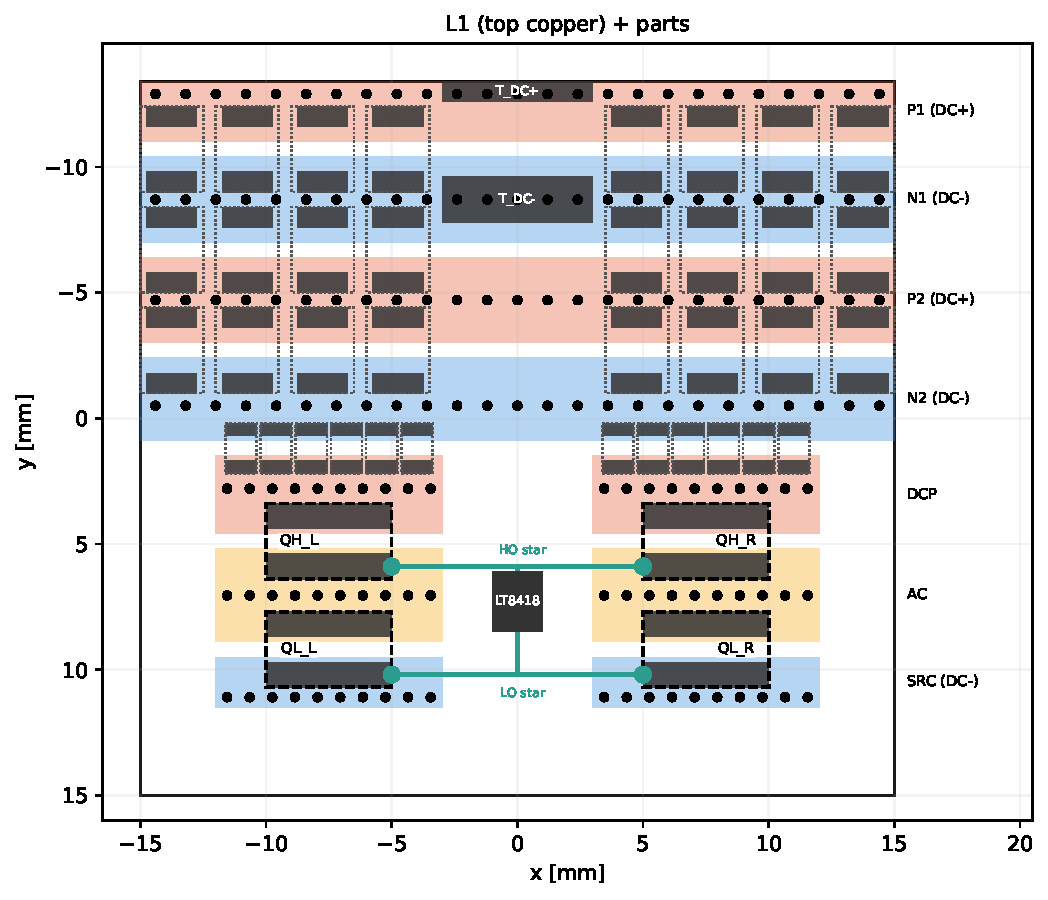
\includegraphics[width=0.78\textwidth]{figures/layout_top.pdf}
\caption{Top layer of the building block (30\,$\times$\,28\,mm). Two mirrored vertical power cells (QH over QL, local MLCCs next to QH) sit at $x=\pm7.5$\,mm; the LT8418 driver is on the symmetry line in a 6\,mm corridor; HO and LO each drive both FETs through an equal star. A 24-part MLCC bank sits above the cells between alternating DC+/DC$-$ strips. Dark rectangles are the pads used as Q3D terminals; dashed outlines are component bodies.}
\label{fig:top}\end{figure}

Every path that matters for current sharing is mirrored about $x=0$: the two commutation loops, the HO and LO gate stars, the DC+ and DC$-$ terminal feeds (on the centre line) and the AC terminal (bottom centre).
The previous studies showed why: a 2.0/7.7\,nH gate-loop mismatch gave a 19\,\% turn-on current imbalance and a 4:1 split of turn-on energy, and unequal common-source inductance was worse still.
Kelvin gate returns are taken at each FET's source pad, so the source inductance is in the power loop only.

\begin{figure}[H]\centering
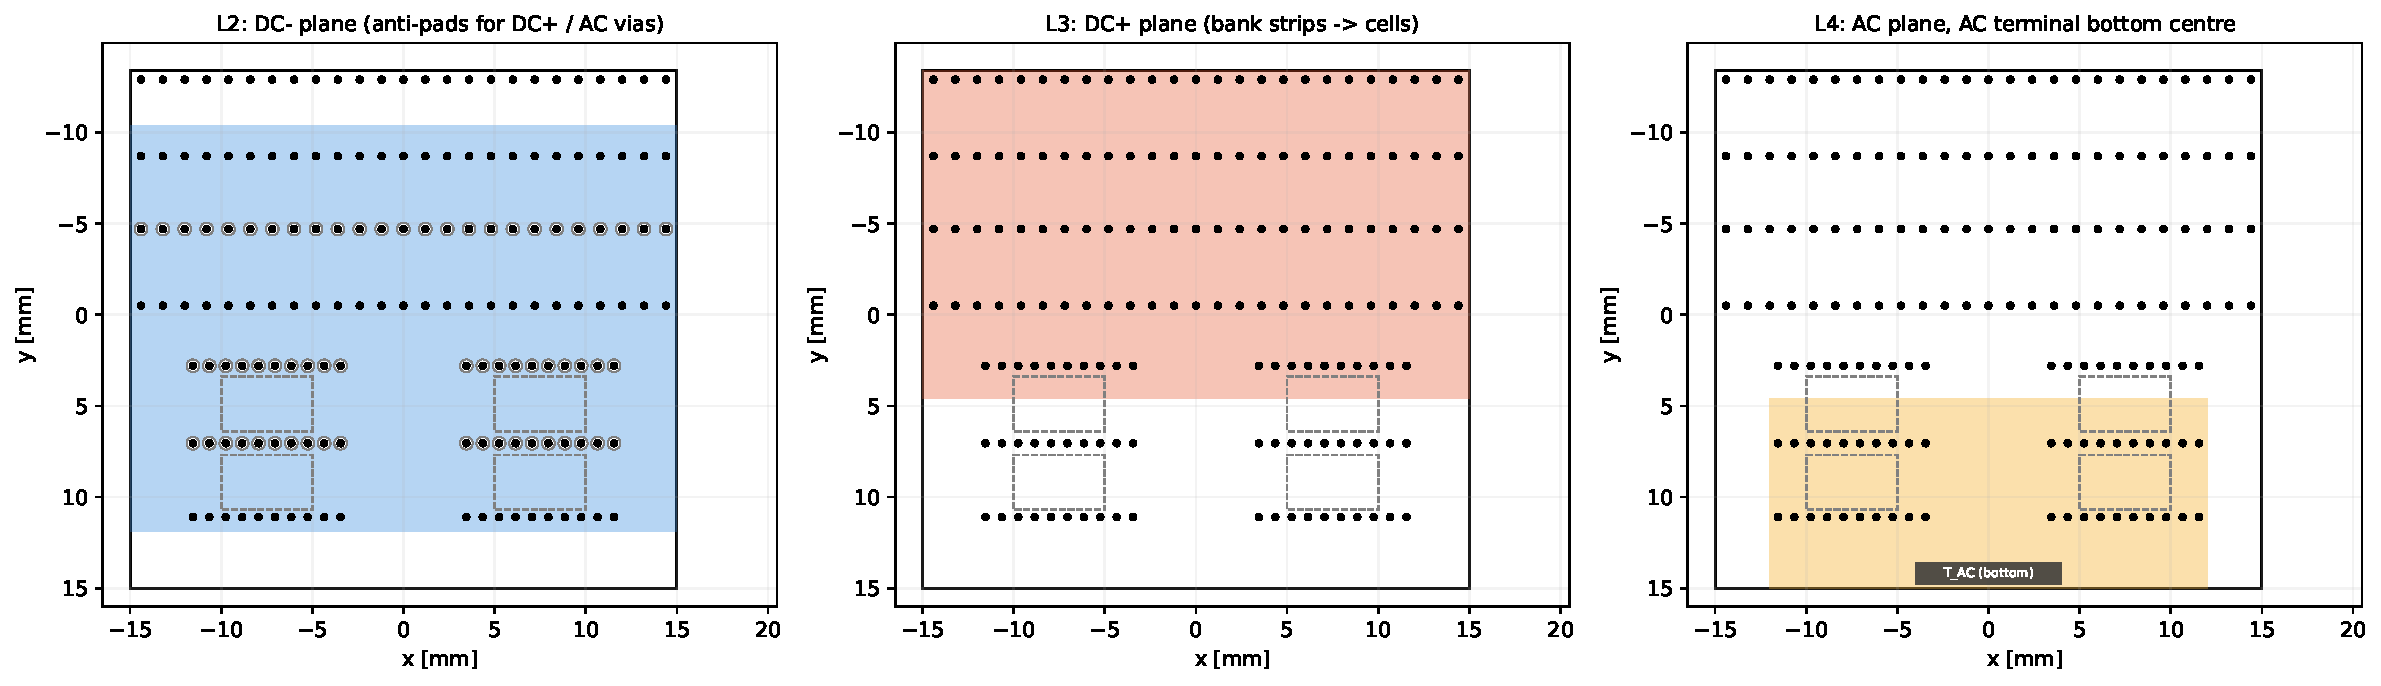
\includegraphics[width=\textwidth]{figures/layout_inner.pdf}
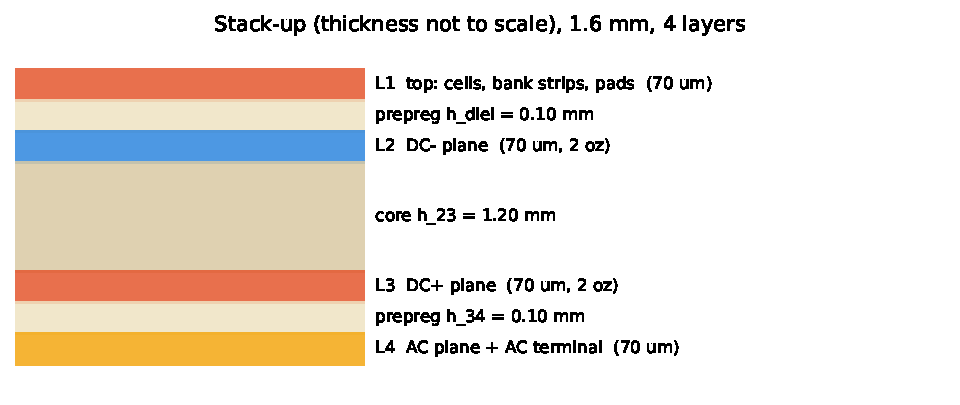
\includegraphics[width=0.62\textwidth]{figures/layout_stackup.pdf}
\caption{Inner and bottom layers and the 4-layer stack-up (2\,oz on all layers, see Section~\ref{sec:cu}). L2 is a solid DC$-$ return 0.1\,mm under the cells (anti-pads only where DC+ and AC vias pass); L3 carries DC+ from the bank strips to both cells; L4 joins both switch nodes to the AC terminal on the bottom side.}
\label{fig:inner}\end{figure}

\section{DC link and auxiliary circuits}\label{sec:dclink}
The DC-link current was computed with an ideal three-phase SVPWM inverter (common triangular carrier, 50\,kHz, 100\,A$_\mathrm{rms}$) over M\,=\,0.1--1.15 and $\cos\varphi$\,=\,0--1 (\texttt{scripts/bb\_sizing.py}).
\begin{itemize}\itemsep0pt
\item HF ripple current of one leg alone: up to \IlegHFworst\,A$_\mathrm{rms}$ (low M, any $\cos\varphi$); \IlegHFrated\,A$_\mathrm{rms}$ at the rated point. This is what a block's own capacitors must be rated for if blocks are physically separated.
\item Three legs sharing one bus: up to \IthreeHF\,A$_\mathrm{rms}$ in total (M\,$\approx$\,0.6, $\cos\varphi$\,=\,1).
\item Effective capacitance for $\pm$2\,\% ripple at 50\,kHz: \CreqTotal\,\uF{} for the shared bus, i.e.\ \CreqBlock\,\uF{} per block; a single leg on its own would need \CreqAlone\,\uF{}. At 100\,kHz these halve.
\end{itemize}
\begin{figure}[H]\centering
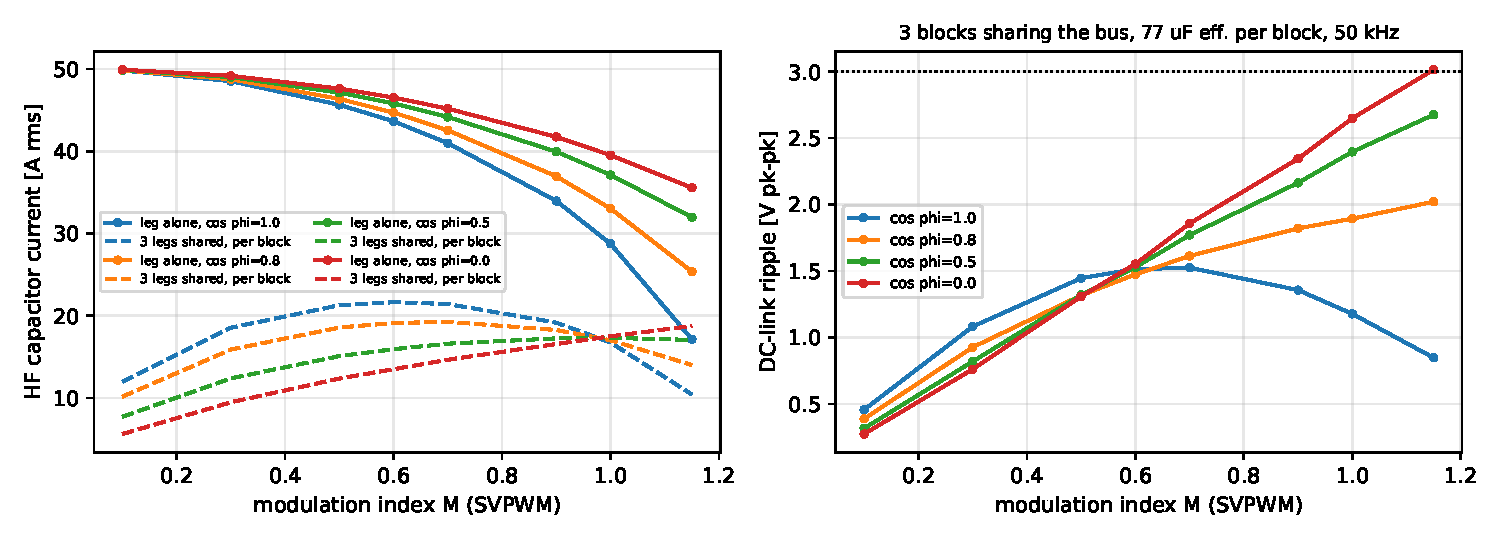
\includegraphics[width=0.9\textwidth]{figures/dc_link_ripple.pdf}
\caption{Left: HF capacitor current per leg (solid: leg alone; dashed: shared bus, per block). Right: DC-link ripple with the selected bank (\CeffBlock\,\uF{} effective per block) on a shared bus.}
\end{figure}

Selected per block: 24\,$\times$ Murata GRM32EC72A106KE05L (10\,\uF{}, 100\,V, X7S, 1210) and 12\,$\times$ TDK C2012X7S2A105K125AB (1\,\uF{}, 100\,V, X7S, 0805, six per cell next to QH).
Assuming 30\,\% and 45\,\% of nominal capacitance at 75\,V (to be checked with the manufacturers' DC-bias data) this gives \CeffBlock\,\uF{} effective, \dVshared\,V peak-peak on a shared bus at 50\,kHz, and \dValone\,V for a leg alone. A stand-alone leg therefore needs additional bulk capacitance (film or polymer) on the DC bus.
The bank ESR loss is \Pcap\,W at the rated point.

\begin{table}[H]\centering\small
\begin{tabular}{@{}lll@{}}\toprule
Function & Part & Sizing \\\midrule
Power switches & 4\,$\times$ EPC2361 & 2 per switch, I$_\mathrm{rms}$ per device \Idev\,A \\
Gate driver & ADI LT8418 (100\,V, 4\,A/8\,A, split outputs, 1.5\,ns matching) & one per block, on the symmetry line \\
Gate resistors & 0402 thin film, per FET R$_\mathrm{g,on}$ = \RgOn\,$\Omega$, R$_\mathrm{g,off}$ = \RgOff\,$\Omega$ & Section~\ref{sec:rg} \\
Bootstrap & 1\,\uF{} 16\,V X7R 0603 (TDK C1608X7R1C105K080AC) & $\geq$\,\CbootMin\,nF for 0.1\,V; droop \BootDroop\,mV with 2\,$\times$\,34\,nC \\
Driver supply & TLV76750 LDO 12\,V$\to$5\,V, 2\,$\times$\,10\,\uF{} + 100\,nF at VCC & gate + LDO loss \Pgate\,W at 50\,kHz \\
Local MLCCs & 12\,$\times$ 1\,\uF{} 100\,V 0805 & commutation loop \\
DC-link bank & 24\,$\times$ 10\,\uF{} 100\,V 1210 & $\pm$2\,\% ripple on a shared bus \\
Logic isolation & TI ISO7720 (shared by the inverter) & controller ground noise \\
\bottomrule\end{tabular}\end{table}

\section{Layout parasitics (Ansys Q3D)}
The geometry of Fig.~\ref{fig:top}--\ref{fig:inner} was built in Q3D Extractor (\texttt{simulation/bb\_q3d}) with the method used for the SiC busbar model: only copper is modelled, every component is a gap with source/sink terminals on its pads, and each copper region is a net (DC+, DC$-$, AC with 18 source and 3 sink terminals). The AC partial-inductance matrix at 100\,MHz is exported as an LTspice subcircuit with coupled inductors. A second design extracts the LO gate star (two branches with Kelvin returns on L2).

\begin{table}[H]\centering\small
\begin{tabular}{@{}lr@{}}\toprule
Commutation loop per cell, copper only (both QL switching, banks ideal) & \LloopCu\,nH \\
\quad incl.\ MLCC ESL (local 6\,$\times$\,0.48\,nH, bank rows 8\,$\times$\,0.5\,nH) & \LloopEsl\,nH \\
\quad local MLCCs only (bank removed) & \LloopLocalEsl\,nH \\
\quad with 2\,oz inner layers & \LloopTwoOz\,nH \\
Gate loop per FET (star branch, one FET driven / both driven) & \LgateOne\,/\,\LgateBoth\,nH \\
DC resistance, AC path (both cells, 2\,oz) & \RacPath\,m$\Omega$ \\
DC resistance, DC+ / DC$-$ path from the terminals (both cells, 1\,oz $\to$ 2\,oz) & \RdcpPathOneOz\,/\,\RdcnPathOneOz\,$\to$\,\RdcpPath\,/\,\RdcnPath\,m$\Omega$ \\
\bottomrule\end{tabular}\end{table}
The EPC2361 package inductance is not included. The mirrored geometry gives identical left and right values (difference $<$\,0.1\,\%). The commutation loop is the same as the single-cell study (0.39\,nH including ESL), so the second cell and the bank do not degrade it; the bank lowers it slightly. The HO star is assumed equal to the extracted LO star (it is 1\,mm shorter).

\subsection*{PCB copper loss}\label{sec:cu}
The DC+ and DC$-$ planes carry the switching-period average current $d\cdot i$ (\IdcpRms\,A$_\mathrm{rms}$ at the rated point) from the terminals above the bank to the cells, 15--20\,mm away; the AC path carries the full 100\,A$_\mathrm{rms}$. With the Q3D DC resistance matrix:
\begin{itemize}\itemsep0pt
\item 1\,oz (35\,\textmu m) inner layers: \PcuOneOz\,W --- more than a third of the loss budget.
\item 2\,oz (70\,\textmu m) inner layers (adopted): \Pcu\,W (AC \PcuAC\,W, DC+ \PcuDCP\,W, DC$-$ \PcuDCN\,W). The loop inductance is unchanged.
\item Further reductions if needed: DC busbar contacts next to each cell instead of above the bank, 3\,oz outer layers for the AC path, or an AC busbar clip directly on the L1 AC islands.
\end{itemize}

\section{Gate resistor selection}\label{sec:rg}
The LTspice model (\texttt{simulation/bb\_spice}) uses the Q3D power-loop and gate-star subcircuits, four EPC2361 models, the capacitor banks with ESR/ESL, a 20\,nH lab busbar with 1\,mF bulk, and an LT8418-like driver (0.6\,$\Omega$ pull-up, 0.2\,$\Omega$ pull-down, split outputs). A low-side double pulse at 160\,A (13\,\% above the 141\,A peak) was swept over R$_\mathrm{g,on}$\,=\,0.5--4\,$\Omega$ and R$_\mathrm{g,off}$\,=\,0--1\,$\Omega$ per FET.
Acceptance: peak V$_\mathrm{DS}$ $\leq$ 90\,V for both devices, off-state V$_\mathrm{GS}$ bump on the complementary FET $\leq$ 1.0\,V, and V$_\mathrm{GS}$ $\geq$ $-$3\,V; among the acceptable pairs the one with the lowest E$_\mathrm{on}$+E$_\mathrm{off}$ is chosen.

\begin{figure}[H]\centering
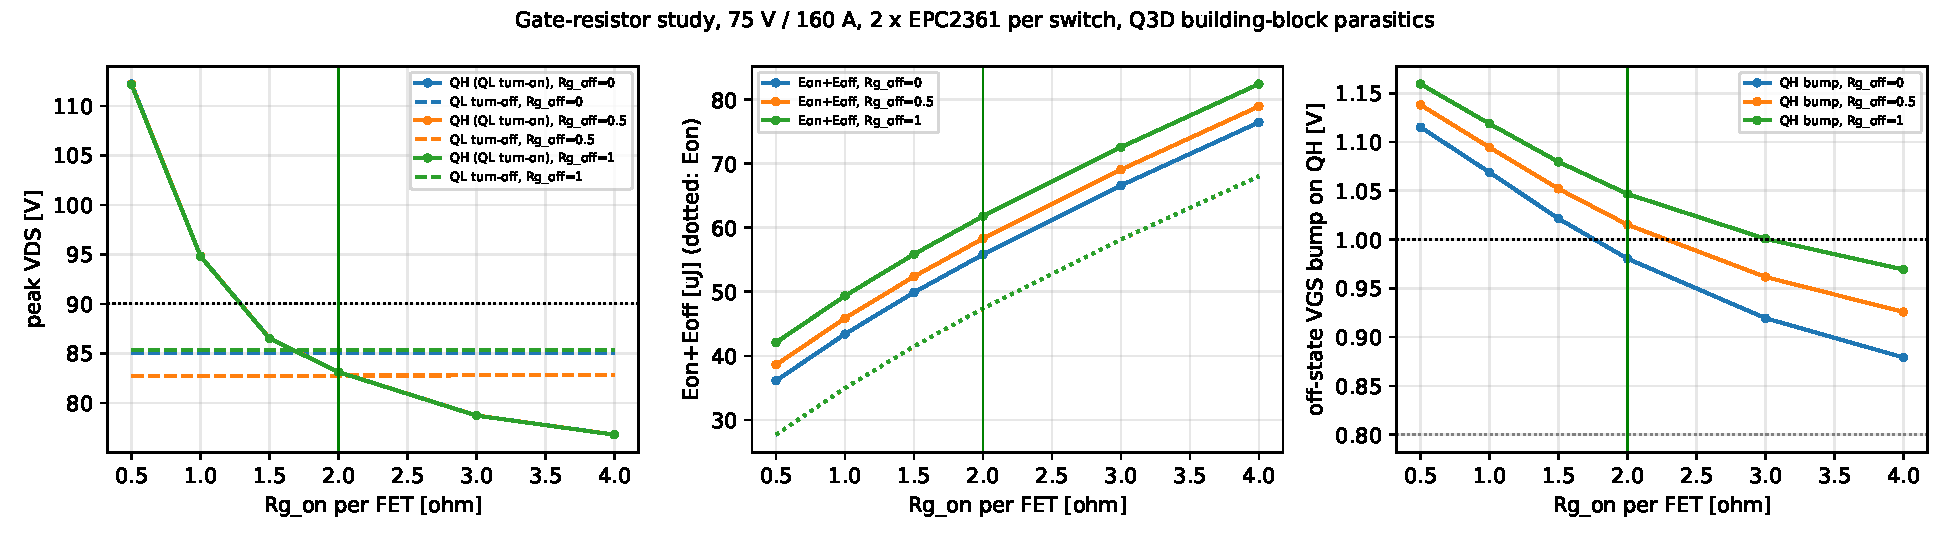
\includegraphics[width=\textwidth]{figures/rg_study.pdf}
\caption{Gate-resistor study at 75\,V / 160\,A. Green line: selected R$_\mathrm{g,on}$.}
\end{figure}

\textbf{Selection: R$_\mathrm{g,on}$\,=\,\RgOn\,$\Omega$, R$_\mathrm{g,off}$\,=\,\RgOff\,$\Omega$ per FET.} At 160\,A: QH peak \VdsH\,V, QL peak \VdsL\,V, QH gate bump \VgsBump\,V, minimum V$_\mathrm{GS}$ \VgsMin\,V, E$_\mathrm{on}$\,=\,\EonPk\,\textmu J and E$_\mathrm{off}$\,=\,\EoffPk\,\textmu J per switch position, dv/dt \DvdtOn\,V/ns (turn-on) and \DvdtOff\,V/ns (turn-off).
R$_\mathrm{g,on}\geq$\,1.5\,$\Omega$ is needed for the 90\,V limit (1\,$\Omega$ gives 95\,V, 0.5\,$\Omega$ 112\,V), and 2\,$\Omega$ for the gate-bump limit; R$_\mathrm{g,off}$ = 0 gives the lowest E$_\mathrm{off}$ and the smallest bump. Turn-off is load-driven at these currents (E$_\mathrm{off}$ $\approx$ 7--8\,\textmu J over the whole current range). The 0.98\,V bump is just above the 0.8\,V minimum threshold but below the 1.1\,V typical; it lasts about 4\,ns. Check the high-side gate on the first double-pulse board; a lower high-side gate-loop inductance is the cure if it causes shoot-through. The dv/dt values are 20--80\,\% averages and are affected by ringing; if a dv/dt limit is needed (motor insulation, EMI; EPC9186 limits to 10\,V/ns), R$_\mathrm{g,on}$ is the knob, at the cost of E$_\mathrm{on}$.

\begin{figure}[H]\centering
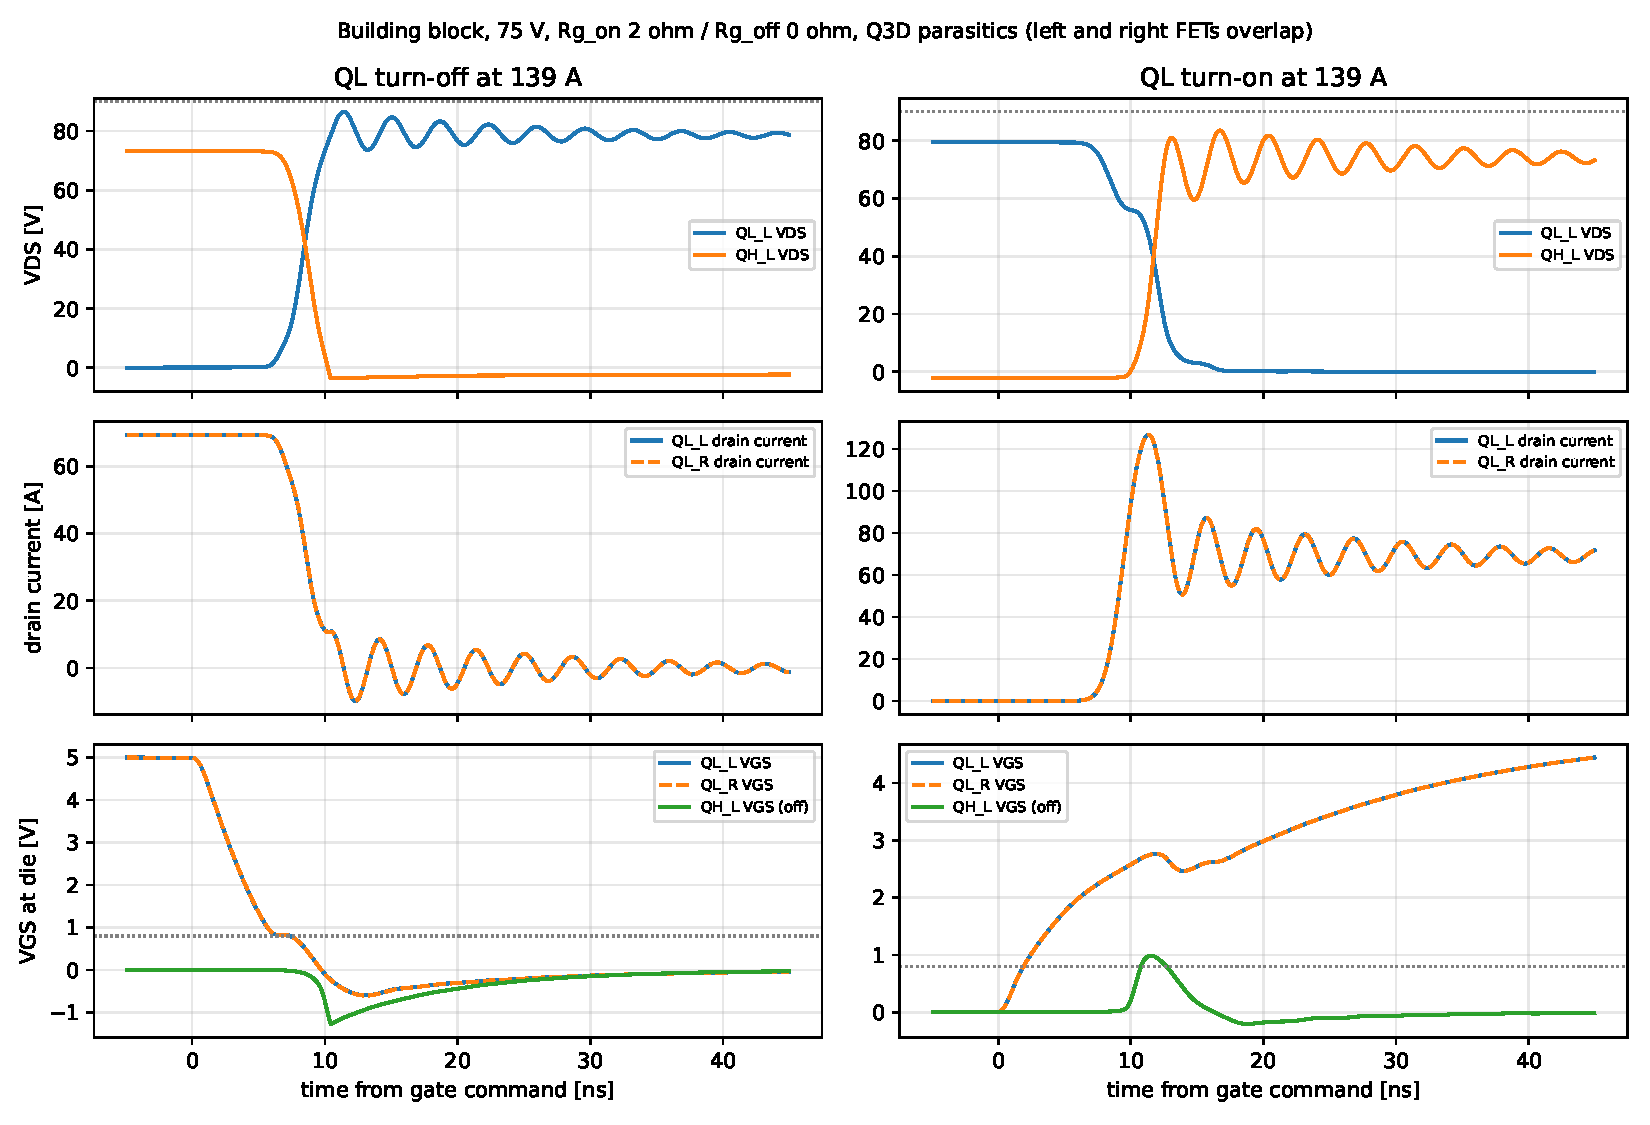
\includegraphics[width=0.95\textwidth]{figures/waveforms_141A.pdf}
\caption{Switching at the rated peak current with the selected resistors. The left and right FETs (solid and dashed) overlap: the symmetric layout shares current equally at both edges.}
\end{figure}

\section{Losses and efficiency}
The switching energy versus current was simulated with the selected resistors and fitted with second-order polynomials; the inverter switching loss is $P_\mathrm{sw}=f_\mathrm{sw}\,\frac{1}{\pi}\int_0^\pi\left[E_\mathrm{on}+E_\mathrm{off}\right](I_\mathrm{pk}\sin\theta)\,d\theta$ (average \Eavg\,\textmu J per period).

\begin{figure}[H]\centering
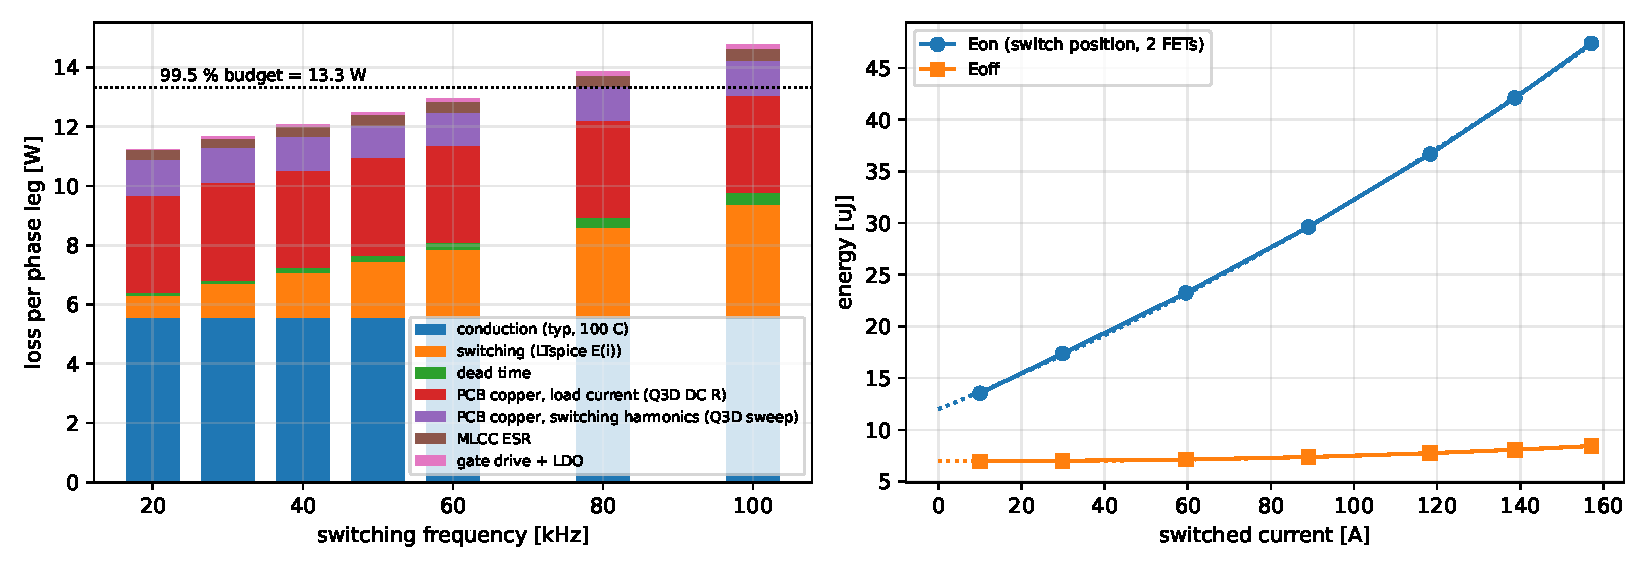
\includegraphics[width=\textwidth]{figures/losses.pdf}
\caption{Left: loss per phase leg versus switching frequency at the rated point. Right: switching energy per switch position (two FETs) versus current, LTspice with Q3D parasitics.}
\end{figure}

\begin{table}[H]\centering\small
\begin{tabular}{@{}lr@{}}\toprule
Loss component at 50\,kHz, rated point & W \\\midrule
Conduction, R$_\mathrm{DS(on)}$ typ at 100\,$^\circ$C ($I^2 R_\mathrm{DS}/2$) & \PcondTyp \\
Switching (LTspice E(i), selected R$_\mathrm{g}$) & \Psw \\
Dead time (2\,$\times$\,10\,ns per period, reverse conduction) & \Pdead \\
PCB copper (Q3D DC resistance) & \Pcu \\
DC-link ESR & \Pcap \\
Gate drive + LDO & \Pgate \\\midrule
\textbf{Total} & \textbf{\Ptot} \\
\textbf{Efficiency} (budget \Pbudget\,W) & \textbf{\Eta\,\%} \\
With R$_\mathrm{DS(on)}$ max at 100\,$^\circ$C & \PtotWorst\,W, \EtaWorst\,\% \\
\bottomrule\end{tabular}\end{table}
The 99.5\,\% target is met over 20--100\,kHz with typical devices; at 100\,kHz the loss (13.3\,W) equals the budget, so 50\,kHz leaves margin for device spread (\PtotWorst\,W with maximum R$_\mathrm{DS(on)}$). E$_\mathrm{on}$ does not go to zero at zero current: charging the high-side output capacitance through the low-side channel costs about Q$_\mathrm{oss}$V\,$\approx$\,2\,$\times$\,113\,nC\,$\times$\,75\,V. Conduction dominates; at 25\,$^\circ$C it would be \PcondCold\,W, so cooling directly reduces loss. Per device the loss is about \Pdev\,W at 50\,kHz; with 0.2\,K/W junction-to-case, an insulating TIM of about 1.9\,K/W per device and a 60\,$^\circ$C heat sink, T$_\mathrm{j}\approx$\,\Tj\,$^\circ$C. The conduction loss above assumes 100\,$^\circ$C, so this is conservative.

\section{Limitations and next steps}
\begin{itemize}\itemsep0pt
\item MLCC capacitance under 75\,V DC bias is assumed (30\,\% / 45\,\%); confirm with Murata SimSurfing and TDK data before freezing the bank.
\item The Q3D model is a pre-layout geometry with simplified two-bar FET pads; repeat the extraction on the routed KiCad board. Package inductance and frequency-dependent resistance are not in the SPICE model, so ringing is under-damped.
\item Losses use typical device parameters and a 10\,ns dead time; switching energy comes from a model, not a measurement. Validate with the double-pulse board.
\item Thermal design (TIM, heat sink, coolant) is only estimated; the per-device budget above sets its requirement.
\end{itemize}

\textbf{Files.} Sizing \texttt{scripts/bb\_sizing.py}; geometry \texttt{simulation/bb\_q3d/bb\_geometry.py}; Q3D \texttt{simulation/bb\_q3d/bb\_q3d.py}; LTspice \texttt{simulation/bb\_spice/}; results and this report's numbers \texttt{scripts/bb\_losses.py}; layout page \texttt{docs/building-block-layout.html}.
\end{document}
